\documentclass[10pt]{article}

%%%%%%%%%%%%%%%%%%%%%%%%%%%%%%%%%%%%%%%%%%%%%%%%%%%%%%%%%%%%%%%%%%%%%%%%%%%%%%%%
% LaTeX Imports
%%%%%%%%%%%%%%%%%%%%%%%%%%%%%%%%%%%%%%%%%%%%%%%%%%%%%%%%%%%%%%%%%%%%%%%%%%%%%%%%
\usepackage{amsfonts}                                                   % Math fonts
\usepackage{amsmath}                                                    % Math formatting
\usepackage{amssymb}                                                    % Math formatting
\usepackage{amsthm}                                                     % Math Theorems
\usepackage{arydshln}                                                   % Dashed hlines
\usepackage{attachfile}                                                 % AttachFiles
\usepackage{cancel}                                                     % Cancelled math
\usepackage{caption}                                                    % Figure captioning
\usepackage{color}                                                      % Nice Colors
\input{./lib/dragon.inp}                                                % Tikz dragon curve
\usepackage[ampersand]{easylist}                                        % Easy lists
\usepackage{fancyhdr}                                                   % Fancy Header
\usepackage[T1]{fontenc}                                                % Specific font-encoding
%\usepackage[margin=1in, marginparwidth=2cm, marginparsep=2cm]{geometry} % Margins
\usepackage{graphicx}                                                   % Include images
\usepackage{hyperref}                                                   % Referencing
\usepackage[none]{hyphenat}                                             % Don't allow hyphenation
\usepackage{lipsum}                                                     % Lorem Ipsum Dummy Text
\usepackage{listings}                                                   % Code display
\usepackage{marginnote}                                                 % Notes in the margin
\usepackage{microtype}                                                  % Niceness
\usepackage{lib/minted}                                                 % Code display
\usepackage{multirow}                                                   % Multirow tables
\usepackage{pdfpages}                                                   % Include pdfs
\usepackage{pgfplots}                                                   % Create Pictures
\usepackage{rotating}                                                   % Figure rotation
\usepackage{setspace}                                                   % Allow double spacing
\usepackage{subcaption}                                                 % Figure captioning
\usepackage{tikz}                                                       % Create Pictures
\usepackage{tocloft}                                                    % List of Equations
%%%%%%%%%%%%%%%%%%%%%%%%%%%%%%%%%%%%%%%%%%%%%%%%%%%%%%%%%%%%%%%%%%%%%%%%%%%%%%%%
% Package Setup
%%%%%%%%%%%%%%%%%%%%%%%%%%%%%%%%%%%%%%%%%%%%%%%%%%%%%%%%%%%%%%%%%%%%%%%%%%%%%%%%
\hypersetup{%                                                           % Setup linking
    colorlinks=true,
    linkcolor=black,
    citecolor=black,
    filecolor=black,
    urlcolor=black,
}
\RequirePackage[l2tabu, orthodox]{nag}                                  % Nag about bad syntax
\renewcommand*\thesection{\arabic{section} }                             % Reset numbering
\renewcommand{\theFancyVerbLine}{ {\arabic{FancyVerbLine} } }              % Needed for code display
\renewcommand{\footrulewidth}{0.4pt}                                    % Footer hline
\setcounter{secnumdepth}{3}                                             % Include subsubsections in numbering
\setcounter{tocdepth}{3}                                                % Include subsubsections in toc
%%%%%%%%%%%%%%%%%%%%%%%%%%%%%%%%%%%%%%%%%%%%%%%%%%%%%%%%%%%%%%%%%%%%%%%%%%%%%%%%
% Custom commands
%%%%%%%%%%%%%%%%%%%%%%%%%%%%%%%%%%%%%%%%%%%%%%%%%%%%%%%%%%%%%%%%%%%%%%%%%%%%%%%%
\newcommand{\nvec}[1]{\left\langle #1 \right\rangle}                    %  Easy to use vector
\newcommand{\ma}[0]{\mathbf{A} }                                         %  Easy to use vector
\newcommand{\mb}[0]{\mathbf{B} }                                         %  Easy to use vector
\newcommand{\abs}[1]{\left\lvert #1 \right\rvert}                       %  Easy to use abs
\newcommand{\pren}[1]{\left( #1 \right)}                                %  Big parens
\let\oldvec\vec
\renewcommand{\vec}[1]{\oldvec{\mathbf{#1} } }                            %  Vector Styling
\newtheorem{thm}{Theorem}                                               %  Define the theorem name
\newtheorem{definition}{Definition}                                     %  Define the definition name
\definecolor{bg}{rgb}{0.95,0.95,0.95}
\newcommand{\java}[4]{\vspace{10pt}\inputminted[firstline=#2,
                                 lastline=#3,
                                 firstnumber=#2,
                                 gobble=#4,
                                 frame=single,
                                 label=#1,
                                 bgcolor=bg,
                                 linenos]{java}{#1} }
\newcommand{\python}[4]{\vspace{10pt}\inputminted[firstline=#2,
                                 lastline=#3,
                                 firstnumber=#2,
                                 gobble=#4,
                                 frame=single,
                                 label=#1,
                                 bgcolor=bg,
                                 linenos]{python}{#1} }
\newcommand{\js}[4]{\vspace{10pt}\inputminted[firstline=#2,
                                 lastline=#3,
                                 firstnumber=#2,
                                 gobble=#4,
                                 frame=single,
                                 label=#1,
                                 bgcolor=bg,
                                 linenos]{js}{#1} }
%%%%%%%%%%%%%%%%%%%%%%%%%%%%%%%%%%%%%%%%%%%%%%%%%%%%%%%%%%%%%%%%%%%%%%%%%%%%%%%%
% Beginning of document items - headers, title, toc, etc...
%%%%%%%%%%%%%%%%%%%%%%%%%%%%%%%%%%%%%%%%%%%%%%%%%%%%%%%%%%%%%%%%%%%%%%%%%%%%%%%%
\pagestyle{fancy}                                                       %  Establishes that the headers will be defined
\fancyhead[LE,LO]{Computer Systems Notes}                                  %  Adds header to left
\fancyhead[RE,RO]{Zoe Farmer}                                       %  Adds header to right
\cfoot{ \thepage }
\lfoot{CSCI 2400}
\rfoot{Han}
\title{Computer Systems Notes}
\author{Zoe Farmer}

%%%%%%%%%%%%%%%%%%%%%%%%%%%%%%%%%%%%%%%%%%%%%%%%%%%%%%%%%%%%%%%%%%%%%%%%%%%%%%%%
% Beginning of document items - headers, title, toc, etc...
%%%%%%%%%%%%%%%%%%%%%%%%%%%%%%%%%%%%%%%%%%%%%%%%%%%%%%%%%%%%%%%%%%%%%%%%%%%%%%%%
\pagestyle{fancy}                                                       %  Establishes that the headers will be defined
\fancyhead[LE,LO]{Problem Set 1}                                  %  Adds header to left
\fancyhead[RE,RO]{Zoe Farmer}                                       %  Adds header to right
\cfoot{ \thepage }
\lfoot{CSCI 3104}
\rfoot{Clauset}
\title{Problem Set One}
\author{Zoe Farmer}
%%%%%%%%%%%%%%%%%%%%%%%%%%%%%%%%%%%%%%%%%%%%%%%%%%%%%%%%%%%%%%%%%%%%%%%%%%%%%%%%
% Beginning of document items - headers, title, toc, etc...
%%%%%%%%%%%%%%%%%%%%%%%%%%%%%%%%%%%%%%%%%%%%%%%%%%%%%%%%%%%%%%%%%%%%%%%%%%%%%%%%
\begin{document}

\maketitle

\begin{easylist}[enumerate]
    @ \textit{For each claim, determine whether the statement is \textbf{True} or \textbf{False}. Justify your answer.}
    @@ $ n + 3 = O(n^3) \to $ \textbf{True}. According to the definition of Big-O notation, $f = O(g)$ if
        \[ \left( \exists c, k > 0, x > k \right) \left[ \abs{f(x)} \le c \abs{g(x)} \right] \]
        Therefore
        \[ \boxed{\abs{n+3} \le c \abs{n^3} } \]
        and the statement is valid.
    @@ $ 3^{2n} = O(3^n) \to $ \textbf{False}. Again, using the previous definition of Big-O notation we see that
        \[ \boxed{\abs{3^{2n} } \not\le c \abs{3^n} } \]
    @@ $ n^n = o(n!) \to $ \textbf{False}. We can use the definition of little-o notation which states that $f$ is little-o of $g$ if
        \[ \lim_{x\to\infty} \frac{f(x)}{g(x)} = 0 \]
        Therefore this statement turns to
        \[ \boxed{\lim_{x\to\infty} \frac{n^n}{n!} = \infty} \]
        Therefore the statement is invalid.
    @@ $ \frac{1}{3n} = o(1) \to $ \textbf{True}. We then use the above definition again and apply L'Hospital's Rule to determine the value of the limit.
        \[ \lim_{x\to\infty} \frac{1}{3n} \to \boxed{\lim_{x\to\infty} \frac{0}{3} = 0} \]
    @@ $ \ln^3(n) = \Theta (\log^3_2(n)) \to $ \textbf{False}\footnote{This is assuming that $lg(x)$ refers to the base-2 logarithm, $\log_2(x)$.} We can use the definition of Big-O notation to determine that
        \[ \boxed{\ln^3(n) = O(\log^3_2(n))} \]
        because $\abs{\ln^3(n)} \le c \abs{\log^3_2(n)}$, however
        \[ \boxed{\log^3_2(n) \neq O(\ln^3(n))} \]
        because $\abs{\log^3_2(n)} \not\le c \abs{\ln^3(n)}$. Therefore the statement is false.

    \rule{3in}{0.5pt}

    @ \textit{Simplify each of the following expressions.}
    @@ \[ \frac{d}{dt} (3t^4 + 1/3 t^3 - 7 ) \to \boxed{12t^3 + t^2} \]
    @@ \[ \sum^k_{i=0} 2^i \to 1 + 2 + 4 + \cdots + 2^k \to \boxed{2^{k+1} - 1} \]
    @@ \[ \Theta \left( \sum^n_{k=1} \frac{1}{k} \right) \to \boxed{H_n} \] Where $H_n$ is the $n^{th}$ Harmonic number.

    \rule{3in}{0.5pt}

    @ \textit{$T$ is a balanced binary search tree storing $n$ values. Describe an $O(n)$-time algorithm that takes input $T$ and returns an array containing the same values in \textit{ascending} order.}

    @@ Below is the code to perform this operation.

    \vspace{5pt}\begin{pythoncode*}{gobble=8, label=Balanced Binary Search Tree to Ascending Array}
        asc = []                               # List to populate
        class Node:                            # The structure of any given node
            left = None                        # Class object of left node
            right = None                       # Class object of right node
            value = None                       # Value of node
        def tree_to_array(head):               # Function to scrape in asc order
            if head.left != None:              # If left is node
                tree_to_array(head.left)       # Take left
                head.left = None               # Destroy traversed result
            if head.right != None:             # Else take right
                asc.append(head.value)         # Take next smallest val
                tree_to_array(head.right)      # Go right
                head.right = None              # Destroy traversed result
            if head.left is None and           # If both sides are empty
                    head.right is None:
                try:
                    if (head.value >=
                        asc[len(asc) - 1]):    # If larger than prev
                        asc.append(head.value) # This value is our next smallest
                except IndexError:             # Only enter if list is empty
                    asc.append(head.value)     # This value is our next smallest
        head = construct_tree(random=true)     # Create a random balanced tree
        print(tree_to_array(head))             # Print our end array
    \end{pythoncode*}

    \rule{3in}{0.5pt}

    @ \textit{Acme Corp.\ has asked Professor Flitwick to develop a faster algorithm for their core business. The current algorithm runs in $f(n)$ time. (For concreteness, assume it takes $f(n)$ microseconds to solve a problem of size exactly $n$.) Flitwick believes he can develop a faster algorithm, which takes only $g(n)$ time, but developing it will take $t$ days. Acme only needs to solve a problem of size $n$ once. Should Acme pay Flitwick to develop the faster algorithm or should they stick with their current algorithm? Explain.}
    @@ Let $n = 41, f (n) = 1.99^n , g(n) = n^3$ and $t = 17$ days.
    @@@ The time it will take the original algorithm to complete is
        \[ 1.99^n \text{ where } n=41 \to 1790507451731.9128 ms \to 20.7235 d \]
        Flitwick can complete and run his algorithm in
        \[ 17 + n^3 \text{ where } n=41 \to 17 d + 68921 ms \to 17.0000007977 d \]
        Therefore the company \textit{should} pay him to develop the better algorithm as it will save them 3 days time.
    @@ Let $n = 10^6 , f (n) = n^{2.00} , g(n) = n^{1.99}$ and $t = 2$ days.
    @@@ The time it will take the original algorithm to complete is
        \[ n^{2.00} \text{ where } n=10^6 \to 1000000000000 ms \to 11.5741 d \]
        Flitwick can complete and run his algorithm in
        \[ 2 + n^{1.99} \text{ where } n=10^6 \to 2 d + 870963589956.0806 ms \to 12.0806 d \]
        Therefore the company \textit{should not} pay him to develop the better algorithm as it will take an extra day and a half to complete.

    \rule{3in}{0.5pt}

    @ \textit{Using the mathematical definition of Big-O, answer the following. Show your work.}
    @@ Is $2^{nk} = O(2^n)$ for $k > 1$?
    @@@ No. $2^{nk}$ will always grow faster that $2^n$.
        \[ 2^{nk} \to {(2^n)}^k \to \abs{ {(2^n)}^k} \not\le c \abs{2^n} \]
    @@ Is $2^{n+k} = O(2^n)$, for $k = O(1)$?
    @@@ Yes. $2^k$ is constant, therefore
        \[ 2^{n+k} \to 2^n 2^k \to \vert {2^n \cancelto{c}{2^k} } \vert \le c \abs {2^n} \]

    \rule{3in}{0.5pt}

    @ \textit{Is an array that is in sorted order also a min-heap? Justify.}
    @@ Technically no, they are not the same. They have differing data structures, however they are more similar than not upon further inspection. A sorted array has the form {\ttfamily [1, 2, 3, 4, 5]} while a min-heap has the form

        \begin{figure}[ht]
            \centering
            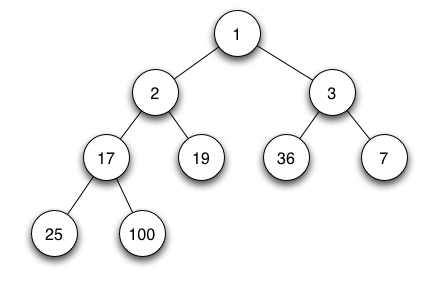
\includegraphics[scale=0.5]{img/Min-heap.png}
            \caption{A Sample Min-Heap}
        \end{figure}

    with a corresponding data structure similar to the sample code below.

    \vspace{5pt}\begin{pythoncode*}{gobble=12, label=Sample Min-Heap Data Structure}
            class Node:
                left = left_node_class_object   # Must be greater than Node
                right = right_node_class_object # Must be greater than Node
                value = node_value
        \end{pythoncode*}

    As is evident the fundamental data structures expressing the two are not similar in the slightest. This being said however, a sorted array will correspond the following min-heap

        \begin{figure}[ht]
            \centering
            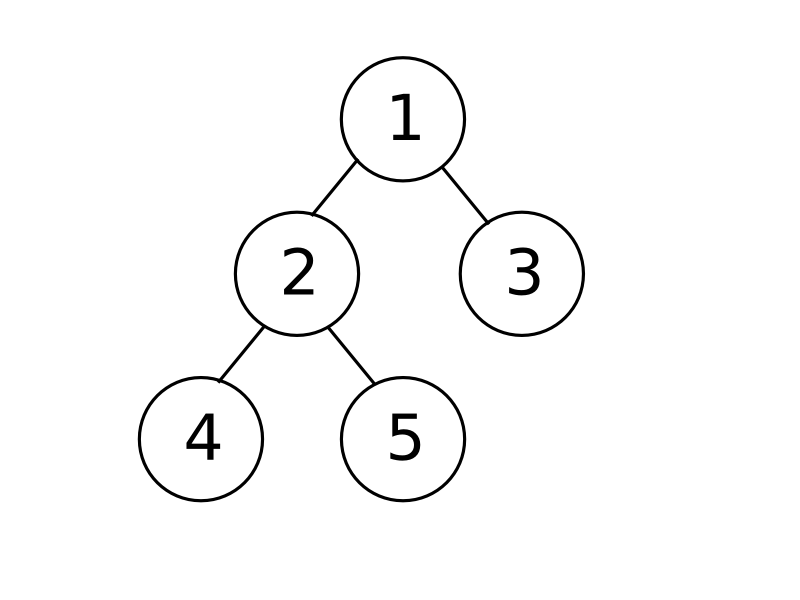
\includegraphics[scale=0.3]{img/minheaparray.png}
            \caption{The Min-Heap for our Array}
        \end{figure}

    When the min-heap is accessed top-down, left-to-right it will have a one-to-one correspondence to our array. So to put it succinctly, the two data structures are not the same, however they have similar appearance and behavior.

\end{easylist}

\end{document}
